%
% The first command in your LaTeX source must be the \documentclass command.
\documentclass[acmsmall]{acmart}
\usepackage{graphicx}
%
% defining the \BibTeX command - from Oren Patashnik's original BibTeX documentation.
\def\BibTeX{{\rm B\kern-.05em{\sc i\kern-.025em b}\kern-.08emT\kern-.1667em\lower.7ex\hbox{E}\kern-.125emX}}
    
\copyrightyear{2020}
\acmYear{2020}
\setcopyright{none}
\acmConference[]{none}
\acmBooktitle{none}
\acmPrice{none}
\acmDOI{none}
\acmISBN{none}

\settopmatter{printacmref=false}
 \setcopyright{none}
 \renewcommand\footnotetextcopyrightpermission[1]{}



\begin{document}

%
% The "title" command has an optional parameter, allowing the author to define a "short title" to be used in page headers.
\title{EULER CIRCUITS AND THE  KÖNIGSBERG BRIDGE PROBLEM}

%
% The "author" command and its associated commands are used to define the authors and their affiliations.
% Of note is the shared affiliation of the first two authors, and the "authornote" and "authornotemark" commands
% used to denote shared contribution to the research.
\author{Anshu Singh (185035)}
\authornote{All team members contributed equally to this documentation.}
\email{185035@nith.ac.in}
\affiliation{%
  \institution{ National Institute of Technology, Hamirpur}
}


\author{Anshudhar Kumar Singh(185032)}
%\authornotemark[1]
\email{185032@nith.ac.in}
\affiliation{%
  \institution{ National Institute of Technology, Hamirpur}
}

\author{Anshika (185041)}
\email{185041@nith.ac.in}
\affiliation{%
  \institution{ National Institute of Technology, Hamirpur}
}

%
% By default, the full list of authors will be used in the page headers. Often, this list is too long, and will overlap
% other information printed in the page headers. This command allows the author to define a more concise list
% of authors' names for this purpose.
\renewcommand{\shortauthors}{}

%
% The abstract is a short summary of the work to be presented in the article.
\begin{abstract}
The Seven Bridges of Königsberg is a historically notable problem in mathematics. Its negative resolution by Leonhard Euler in 1736[1] laid the foundations of graph theory and prefigured the idea of topology.

The city of Königsberg in Prussia (now Kaliningrad, Russia) was set on both sides of the Pregel River, and included two large islands—Kneiphof and Lomse—which were connected to each other, or to the two mainland portions of the city, by seven bridges. The problem was to devise a walk through the city that would cross each of those bridges once and only once.

Euler proved that the problem has no solution. The difficulty he faced was the development of a suitable technique of analysis, and of subsequent tests that established this assertion with mathematical rigor.
\end{abstract}

%
% Please copy and paste the code instead of the example below.
%

%
% Keywords. The author(s) should pick words that accurately describe the work being
% presented. Separate the keywords with commas.
\keywords{Euler circuit, königsberg bridge problem, graph theory, research paper summary}

%
%
% This command processes the author and affiliation and title information and builds
% the first part of the formatted document.
\maketitle

\section{Introduction}
Modern graph theory has seen many developments throughout the centuries, yet the remarkable beginning of graph theory was a ‘feeble glance’ which Leonard Euler directed towards the geometry of position. Euler undertook the development of mathematical formulation of now-famous as The Konigsberg Bridge Problem in his paper Commentarii Academiae Scientiarum Im- perialis Petropolitanae in 1736.

\section{Königsberg}
The story started in the town of Königsberg, Prussia on the banks of Pregel River. In the Middle Ages, Königsberg became a very important city and trading center. The healthy economy allowed the people of the city to build seven bridges across the river. The river divided the city into four regions. And according to lore, the people of the city decide to create a game with the goal being to devise a way in which they could walk around the city, through each bridge exactly once.\\

Though the problem has the appearance of an interesting puzzle, it does not involve measurements nor calculations. As first stated as Leibniz’s “geometry of position” , Euler suggested that the solution to the problem of the bridges only included position and hence was an example of the geometry of position. Euler introduces and utilizes now called
graph theory in solving this famous problem. From such deceptively frivolous origins, graph theory grew into a powerful and deep mathematical theory.


\begin{figure}[h]
  \centering
  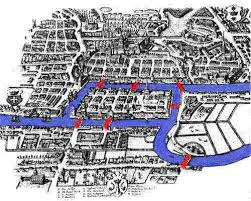
\includegraphics[width=\linewidth]{koncity}
  \caption{The city of Königsberg.}
  \Description{The city of Königsberg.}
\end{figure}



\section{Euler's Methodology}

Euler states the problem as follows :

“in Königsberg in Prussia, there is an island A , called the Kneiphof ; the river which surrounds it is
divided into two branches, as can be seen in Fig. [1], and these branches are crossed by seven bridges,
a,b,c,d,e,f and g . Concerning these bridges, it was asked whether anyone could arrange a route in such a
way that he would cross each bridge once and only once. ”\\


He first generalised the problem as :

“ whatever be the arrangement and division of the river into branches, and however many bridges there be,
can one find out whether or not it is possible to cross each bridge exactly once? ”\\


He began his analysis by replacing the land with points and bridges with line segments. He
started with first ruling out the choice of making exhaustive lists of all possible routes as this task was too difficult as well as laborious. Hence, he first tries to find if there is such a path or not?\\


He then starts to name the land using capital letters and writes the route as follows;

“If a traveller goes from A to B over bridge a or b , I write this as AB — where the first letter refers to the
area the traveller is leaving, and the second refers to the area he arrives at after crossing the bridge. Thus, if
the traveller leaves B and crosses into D over bridge f , this crossing is represented by BD , and the two
crossing AB and BD combined I shall denote by the three letters ABD , where the middle letter B refers to
both the area which is entered in the first crossing and to the one which is left in the second crossing.”\\

And hence by this method it was observed that for representing n bridges we need (n+1)
points. If we can do that it means such a route will be possible.\\

And hence the modern day definition of walk i.e. a sequence of alternating vertices and
edges in which both the order of vertices and edges used are specified. And if no edge is
repeated, it is said to be path and if the terminal and initial vertex are equal, the path is
said to be circuit.\\

The problem was therefore reduced to finding a sequence of letters. But before this euler
turned to a sub problem that is, if there is such a sequence even possible?\\

For this purpose he turned to a rule where he only considered two areas, and tried to find
out occurrences of landmass for different numbers of bridges.\\

\begin{figure}[h]
  \centering
  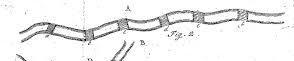
\includegraphics[width=\linewidth]{1t}
  \caption{City with two landmasses.}
  \Description{City with two landmasses.}
\end{figure}


In the figure above, Letter A would occur one time if one bridge is considered, whether he
starts from the A or not. If three bridges are considered, then A will occur twice in sequence
and thrice if number of bridge is five and so on.\\

Hence, if bridges are odd in number then, letter will occur (n+1)/2 times.\\

Similarly on observing the even cases, letter A will occur n/2 times if it started from other
end and (n/2 + 1) times if start from A. (n refers to the number of bridges)\\

And hence, the table for Königsberg bridges will be as follows :
No of Bridges : 7;

\begin{table}[h!]
  \caption{For Königsberg bridges}
  \label{tab:first}
  \begin{tabular}{c c c}
    \toprule
    Region&No of Bridges& No of times one region must occur\\
    \midrule
    A & 5& 3\\
    B & 3& 2\\
    C & 3& 2\\
    D & 3& 2\\
  \bottomrule
\end{tabular}
\end{table}

However, 3+2+2+2 = 9, which is more than 8, so the journey is impossible .\\
Now the same logic applied to a rather following figure, the table yield is as follows :\\

\begin{figure}[h]
  \centering
  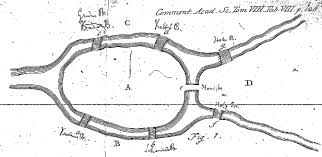
\includegraphics[width=\linewidth]{1}
  \caption{Euler's Imaginary city}
  \Description{Euler's Imaginary city}
\end{figure}


\begin{table}[h!]
  \caption{For Fig.2 bridges}
  \label{tab:sec}
  \begin{tabular}{c c c}
    \toprule
    Region&No of Bridges& No of times one region must occur\\
    \midrule
    A* & 8& 4\\
    B* & 4& 2\\
    C* & 4& 2\\
    D &  3& 2\\
    E &  5& 3\\
    F* & 6& 3\\
  
  \bottomrule
\end{tabular}
\end{table}

By addition, we get 16 which equals to the number of bridges plus one, which means
journey is, in fact, possible.\\

Also, if the total number of appearances is equal to the number of bridges plus one,
journey should start from region in which there are odd number of bridges which leads to
it. And if the number is equal to the number of bridges than it must be started from the
even region.\\


\section{Euler’s Conclusions}

In paragraph 16, Euler points out that the total of the numbers listed directly to the right of
the landmasses adds up to twice the total number of bridges. This fact later becomes
known as the handshaking lemma.\\

In Paragraph 17, Euler goes on to state that the sum of all the bridges leading to each
region is even, since half of this number is equal to the total number of bridges. However,
this is impossible if there are an odd number of landmasses with an odd number of
bridges. Therefore, Euler proves that if there are some odd numbers attached to land
masses, there must be an even number of these landmasses.\\

Euler then explains that it is obvious that if there are two landmasses with an odd number
of bridges then the journey will always be possible if the journey starts in one of the
regions with an odd number of bridges. This is because if the even numbers are halved,
and each of the odd ones are increased by one and halved, the sum of these halves will
equal one more then the total number of bridges. However, if there are four or more
landmasses with an odd number of bridges, then it is impossible for there to be a path.
This is because the sum of the halves of the odd numbers plus one along with the sum of
all of the halves of the even numbers will make the sum of the third column greater than
the total number of bridges plus one. Therefore, Euler just proved that there can be at
most two landmasses with an odd number of bridges.\\

Euler gives the three guidelines that someone can use to figure out if a path exists using
each bridge once and only once. First, he claimed if there are more than two landmasses
with an odd number of bridges, then no such journey is possible. Second, if the number of
bridges is odd for exactly two landmasses, then the journey is possible if it starts in one of
the two odd numbered landmasses. Finally, Euler states that if there are no regions with
an odd number of landmasses then the journey can be accomplished starting in any
region. After stating these three facts, Euler concludes his proof with Paragraph 21, which
simply states that after one figures out that a path exists, they still must go through the
effort to write out a path that works. Euler believed the method to accomplish this was
trivial, and he did not want to spend a great deal of time on it. However, Euler did suggest
concentrating on how to get from one landmass to the other, instead of concentrating on
the specific bridges at first.\\
\clearpage

\section{TASK 1}

Sketch the diagram of a graph with 5 vertices and 8 edges to represent the bridge crossing
problem in the following figure.\\

\begin{figure}[h]
  \centering
  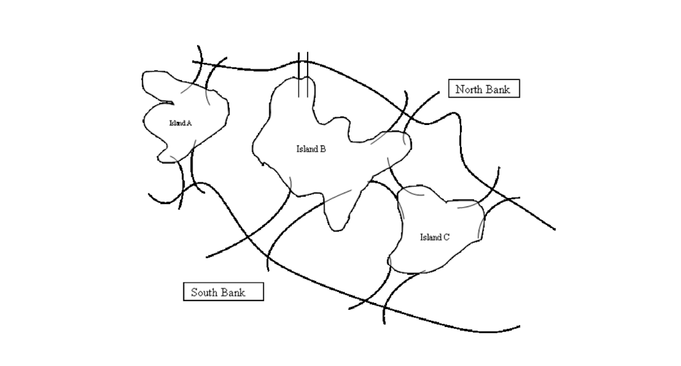
\includegraphics[width=\linewidth]{rsz_13}
  \caption{}
  \Description{}
\end{figure}

For solving the problem we can assume the landmasses as the vertices and the bridges as
the edges. Then we get the following graph :\\

\begin{figure}[h]
  \centering
  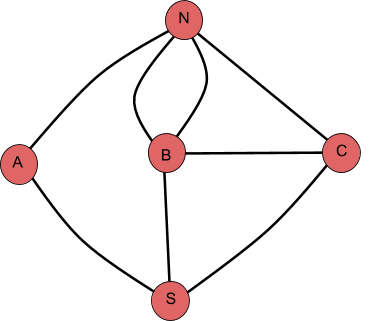
\includegraphics[width=0.5\textwidth]{4}
  \caption{}
  \Description{}
\end{figure}

\clearpage

\section{TASK 2}

For the bridge problem shown in Project TASK 1 above, how many capital letters
(representing graph vertices) will be needed to represent an Euler path?\\
\\
Solution)\\

From Euler’s paragraph 5, it says that we need number of bridges plus one letters for
representing an Euler path.\\

Then according to that we should be needing (8+1) i.e. 9 letters to represent the path.
Also from next paragraphs we can say there would be,

1 times A,

2 times letter B, C, N, S.\\

Hence, in total 9 letters.
\clearpage

\section{TASK 3}

In paragraph 8, Euler deduced a rule for determining how many times a vertex must
appear in the representation of the route for a given bridge problem for the case where an
odd number of bridges leads to the land mass represented by that vertex. Before reading
further, use this rule to determine how many times each of the vertices A , B , C and D
would appear in the representation of a route for the Königsberg Bridge Problem. Given
Euler’s earlier conclusion (paragraph 5) that a solution to this problem requires a sequence
of 8 vertices, is such a sequence possible? Explain.\\
\\
Solution)\\

According to the observation recorded till paragraph 8, Euler found the number of
occurrences of a letter by considering only one landmass as A (the other side of the bridge
will be considered as B).\\

According to that rule, if one crosses one bridge that letter will occur 1 time, if there are
three bridges, then the traveller will have a journey like ABAB or BABA, i.e. two times.
Similarly for five bridges, it should be ABABAB or BABABA. Hence the letter should appear
(n+1)/2 times.\\

Hence, for Königsberg problem, we will have, graph as :
\begin{figure}[h]
  \centering
  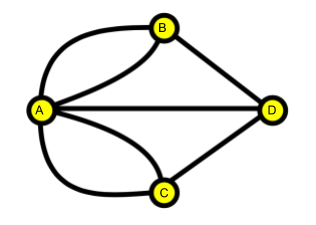
\includegraphics[width=0.5\textwidth]{5}
  \caption{}
  \Description{}
\end{figure}
\\
Hence if we consider each vertices in the above graph, then vertex A have 5 brides, hence it
should occur three times, and since each of the other vertices have three bridges attached
they should occur two times each. Hence the total sequence should be of 3+2+2+2 = 9
digits. But the previous to this statement Euler already proved that the sequence should be
one more than the number of bridges i.e. 8. Hence, such a sequence is not possible. Hence
no Euler path is possible in the Königsberg problem.
\clearpage

\section{References}
   
References used in preparing the document\\

\url{https://google.com}\\


\url{https://medium.com/basecs/k\%C3\%B6nigsberg-seven-small-bridges-one-giant-graph-problem-2275d1670a12}\\


\url{https://www.maa.org/press/periodicals/convergence/leonard-eulers-solution-to-the-konigsberg-bridge-problem#:~:text=Euler\%20states\%20that\%20if\%20the,like\%20the\%20K\%C3\%B6nigsberg\%20Bridge\%20problem}\\


\url{https://scilogs.spektrum.de/hlf/the-bridges-of-konigsberg/}

\end{document}
